\documentclass[11pt, openany]{report}
\usepackage[utf8]{inputenc}
\usepackage[T1]{fontenc}
\usepackage{amsmath,amsfonts,amssymb}
\usepackage{multicol}
\usepackage[a4paper,left=2.5cm,right=2.5cm,top=2.5cm,bottom=2.5cm]{geometry}
\usepackage[english]{babel}
\usepackage{libertine}
\usepackage{gensymb}
\usepackage{tabularray}
\usepackage{nicefrac}
\usepackage{graphicx}
\usepackage{steinmetz}
\usepackage{wrapfig}
\usepackage{float}
\usepackage{algorithm}
\usepackage{algpseudocode}
\usepackage[skins,many]{tcolorbox}
\usepackage{enumitem}
\usepackage{pythonhighlight}
\usepackage{empheq}
\usepackage{mathpazo}
\usepackage{xfrac}
\usepackage{textcomp}
%\usepackage[]{titletoc}
\usepackage{nicematrix}
\usepackage{titlesec}
\usepackage{mathtools}
\usepackage{caption}
\usepackage{subcaption}
\usepackage[bottom]{footmisc}
\usepackage{pdfpages}
\usepackage{tabularx}
\usepackage{amsthm}
\titleformat{\chapter}[display]
  {\normalfont\bfseries}{}{0pt}{\Huge}
\usepackage{hyperref}
\newcommand{\hsp}{\hspace{20pt}}
\newcommand{\HRule}{\rule{\linewidth}{0.5mm}}
\newcommand{\R}{\mathbb{R}}
\newcommand\independent{\protect\mathpalette{\protect\independenT}{\perp}}
\def\independenT#1#2{\mathrel{\rlap{$#1#2$}\mkern2mu{#1#2}}}

\usepackage{apptools}
    \titleformat{\chapter}[hang]{\bfseries\huge}{\IfAppendix{\appendixname~}{\relax}\thechapter\IfAppendix{.}{.}}{\IfAppendix{0.333em}{2pc}}{}

\titlespacing {\chapter}{0pt}{0pt}{40pt}

\usepackage[nottoc]{tocbibind}
\usepackage{keyval}
\usepackage{kvoptions}
\usepackage{fancyvrb}
\usepackage{ifthen}
\usepackage{calc}
\usepackage{pdftexcmds}
\usepackage{etoolbox}
\usepackage{xstring}
\usepackage{xcolor}
\usepackage{lineno}
\usepackage{tikz}
\usepackage{circuitikz}
\usetikzlibrary{patterns,arrows,decorations.pathreplacing,babel}

\usepackage[]{minted}
\newminted{python}{
    linenos=true,
    bgcolor=lightgray,
    tabsize=4,
    gobble=8,
    fontfamily=courier,
    fontsize=\small,
    xleftmargin=5pt,
    xrightmargin=5pt
}

\titleformat{\chapter}[display]
  {\normalfont\bfseries}{}{0pt}{\Huge}

% Define a new tcolorbox style with a red border and transparent interior
\tcbset{
    redbox/.style={
        enhanced,
        colframe=red,
        colback=white,
        boxrule=1pt,
        sharp corners,
        before skip=10pt,
        after skip=10pt,
        box align=center,
        width=\linewidth-2pt, % Adjust the width dynamically
    }
}
\newcommand{\boxedeq}[1]{
\begin{tcolorbox}[redbox]
    \begin{align}
        #1
    \end{align}
\end{tcolorbox}
}
\usepackage[]{titletoc}
\titleformat{\chapter}[display]
  {\normalfont\bfseries}{}{0pt}{\Huge}
\def\independenT#1#2{\mathrel{\rlap{$#1#2$}\mkern2mu{#1#2}}}

\theoremstyle{definition}
\newtheorem{thm}{Theorem}[chapter]
\newtheorem{definition}[thm]{Definition}
\newtheorem{exmp}[thm]{Example} 
\newtheorem{lem}[thm]{Lemma}
\newtheorem{prop}[thm]{Property}
\newtheorem{crl}[thm]{Corollary}
\newtheorem{ex}[thm]{Example}

\usepackage{apptools}
    \titleformat{\chapter}[hang]{\bfseries\huge}{\IfAppendix{\appendixname~}{\relax}\thechapter\IfAppendix{.}{.}}{\IfAppendix{0.333em}{2pc}}{}

\titlespacing {\chapter}{0pt}{0pt}{40pt}


\begin{document}


\begin{titlepage}
    \begin{sffamily}
    \begin{center}
        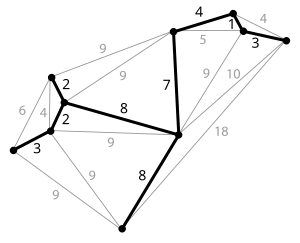
\includegraphics[scale=0.75]{img/page_de_garde.png} \\[1cm]
        \HRule \\[0.4cm]
        { \huge \bfseries LINMA2450 Combinatorial Optimization \\[0.4cm] }
    
        \HRule \\[1.5cm]
        \textsc{\LARGE Simon Desmidt}\\[1cm]
        \vfill
        \vspace{2cm}
        {\large Academic year 2024-2025 - Q1}
        \vspace{0.4cm}
         
        
\includegraphics[width=0.15\textwidth]{img/epl.png}
        
        UCLouvain\\
    
    \end{center}
    \end{sffamily}
\end{titlepage}

\setcounter{tocdepth}{1}
\tableofcontents
\chapter{Introduction}
\section{Continuous vs Combinatorial optimization}
A continuous optimization problem is expressed as 
\begin{equation}\label{eq:1}
    \max/\min f(x)
\end{equation} 
such that \(x\in \Omega\), where \(f:\mathbb{R}^n \rightarrow \mathbb{R}\) and \(\Omega \subseteq \mathbb{R}^n\), where \(\Omega\) does not have isolated points. \\
A combinatorial optimization problem has the additional constraint that \[x\in \Omega \cap \mathbb{Z}^n\] which can be a finite set of values. If finite, it is not solvable by exhaustive search, as it can contain loads of points even for small scale problems.
\section{Upper/Lower bound}
Let \(f^*=\max \{f(x):\quad x\in \Omega\cap \mathbb{Z}^n\}\) be the optimal value for a given problem.
\begin{itemize}
    \item Any lower bound for \(f^*\) is called primal bound. One way to get primal bounds is to find feasible points, because if \(x\in \Omega\cap \mathbb{Z}^n\), then \(f_L = f(x)\le f^*\).
    \item Any upper bound for \(f^*\) is called dual bound. One way to get this upper bound is to use relaxation : \[f^* \le \max_x \{f(x):\quad x\in \Omega\} = f_{\mathcal{U}}\] Thus if \(f_{\mathcal{U}}-f(x)\le \varepsilon\), we have a certificate that \(x\) is an \(\varepsilon\)-approximate solution of \ref{eq:1}.
\end{itemize}
\chapter{Knapsak problem}
Suppose that we have the following : 
\begin{itemize}
    \item a bag;
    \item a set of objects that we want to put in the bag;
    \item each object has a value.
\end{itemize}
The objective of this problem is to select the objects to put in the bag in order to maximze the total value of the objects in the bag, such that the objects fit in the bag. We can only put nonnegative integer amounts of each object in the bag. 
\subsection{Mathematical formulation}
\begin{itemize}
    \item \(b\) : the volume of the bag
    \item \(n\) : the number of types of objects
    \item \(0<a_j\le b\) : the volume of one unit of object \(j\)
    \item \(c_j>0\) : the value of one unit of object \(j\)
    \item \(x_j\) : the amount of object \(j\) that is put in the bag (VARIABLES)
\end{itemize}
The Linear Integer Programming Problem expression here is 
\begin{equation}\label{eq:2}
    \max \sum_{j=1}^n x_jc_j \quad \text{such that}\quad \begin{cases}
        a^Tx \le b\\
        x_j\in \mathbb{N} \quad \forall j=1,\dots,n
    \end{cases}
\end{equation}
Let us now suppose that 
\begin{equation}\label{eq:3}
    \frac{c_1}{a_1}\ge \frac{c_2}{a_2} \ge \dots \ge \frac{c_n}{a_n}
\end{equation}
The greedy approach is to put in the bag the maximum amount possible of object 1, then 2, and so on. The amount of object \(j\) in the bag will therefore be 
\begin{equation}\label{eq:4}
    x_j^{(g)} = \left\lfloor \frac{b-\sum_{i=1}^{j-1} a_ix_i^{(g)}}{a_j} \right\rfloor \quad \forall j=1,\dots,n
\end{equation}
and the feasible point is \(x^{(g)}\) such that it \(j\) component is \(x_j^{(g)}\) calculated above. 
\begin{tcolorbox}[breakable,
                  colback=white,
                  colframe=white!75!black,
                  title={Theorem}]
    Let \(x^{(g)}\) be the feasible point to problem \ref{eq:2} given by the equation \ref{eq:4}, and suppose that the assumption \ref{eq:3} is true. Then,\[f\left(x^{(g)}\right) \ge \sfrac{1}{2} f^*\] that is, the Greedy Heuristics to a Knapsak problem gives a feasible point with a function value equal to at least 50\% of the optimal value.
\end{tcolorbox}
\chapter{Relaxation}
We will here study problems such that the relaxation of the integer constraint still gives the same solution, i.e. solving the discrete or continuous problem is equivalent.\\
\section{Linear problems}
\subsection{Definitions}
\begin{itemize}
    \item A matrix \(B\in \mathbb{Z}^{k\times k}\) is unimodular when it is invertible and \(B^{-1}\in \mathbb{Z}^{k\times k}\). 
    \item \(B\in \mathbb{Z}^{k\times k}\) is unimodular iff \(\det B\in \{-1,1\}\). 
    \item \(A\in \mathbb{Z}^{m\times n}\) is totally unimodular (TU) when every invertible submatrix of \(A\) is unimodular. 
    \item Let \(A\in \mathbb{Z}^{m\times n}\). If \(\det(B) \in \{-1,0,1\}\) for every square submatrix of \(A\), then A is TU.
\end{itemize}
\section{Resolution}\label{sec:main_th}
A linear problem of optimization can be written under the following general form :
\begin{equation}
    \max f(x) = c^Tx \qquad \text{ such that } Ax\le b
\end{equation}
We can use the simplex method in that problem, stating that the solution is one of the vertices of the feasible set (a polygon here). It is possible to rearrange the rows of \(A\) and \(b\) in such a way that we get
\begin{equation}
    \begin{pNiceArray}{c}
  B\\
  \hline
  C\\
\end{pNiceArray} \qquad \begin{pNiceArray}{c}
  b_{(1)} \\
  \hline
  b_{(2)}\\
\end{pNiceArray}
\end{equation}
With that, the solution \(x^* = \begin{pmatrix}
x^*_{(1)}\\ x^*_{(2)}\\ \end{pmatrix}
\) verifies 
\begin{equation}
    \begin{cases}
        Bx_{(1)}^* = b_{(1)}\\
        x_{(2)}^* = 0\\
    \end{cases}
\end{equation}
B being non singular.
\begin{tcolorbox}[breakable,
                  colback=white,
                  colframe=white!75!black,
                  title={Theorem}]
    Let \(A\in \mathbb{Z}^{m\times n}\) be a matrix such that
    \begin{enumerate}
        \item \(A_{ij} \in \{-1,0,1\}\);
        \item Every column of \(A\) has at most 2 nonzero entries:
        \item There exists a partition\footnote{\(I_1\cap I_2 = \emptyset\) and \(I_1 \cup I_2 = \) the set.} \(I_1\cup I_2 = \{1,\dots,m\}\) such that, if the \(j\)th column of \(A\) has exactly 2 nonzero entries, then \(\sum_{i\in I_1} A_{ij} = \sum_{i\in I_2} A_{ij}\);
    \end{enumerate}
    Then \(A\) is TU.
\end{tcolorbox}
\chapter{Applications}
\section{Maximum Matching Problem}
\subsection{Definitions}
\begin{itemize}
    \item Given a graph \(G=(V,E)\), a matching of \(G\) is a subset of edges \(E'\subset E\) such that for every vertex \(v\in V\), there exists at most one edge \(e\in E'\) that is incident to it.
    \item Assume that \(V=\{v_1,\dots,v_m\}\) and \(E=\{e_1,\dots, e_n\}\). Given \(E'\subset E\), we can then associate it to the vector \(x'\in \{0,1\}\subset \mathbb{Z}^n\subset \mathbb{R}^n\) given by 
    \begin{equation}
        x_j' = \begin{cases}
            1 \text{ if } e_j \in E'\\
            0\text{ otherwise}
        \end{cases}
    \end{equation}
    \item Then, with this notation, we have 
    \begin{equation}
        |E'| = \mathbb{1}^Tx'
    \end{equation}
    \item Let us define the vertex-edge incidence matrix of \(G=(V,E)\) as the matrix \(M\in \mathbb{Z}^{m\times n}\) given by
    \begin{equation}
        M_{ij} = \begin{cases} 1 \text{ if }e_j\text{ is incident to }v_j\\ 0 \text{ otherwise}\\ \end{cases} \qquad i=1,\dots,m\qquad j=1,\dots,n
    \end{equation}
\end{itemize}
\subsection{Unweighted Problem}
The maximum unweighted matching problem is to find a subgraph of a bipartite graph for which the maximum number of nodes are related to max one other node. It can be expressed in an combinatorial optimization manner such as:
\begin{equation}
    \max \mathbb{1}^Tx \qquad \text{ such that } Mx\le \mathbb{1}_m \qquad x\in \{0,1\}^n
\end{equation}
We want to be able to use the theorem of section \ref{sec:main_th}. 
\begin{tcolorbox}[breakable,
    colback=white,
    colframe=white!75!black,
    title={Theorem}]
If \(G=(V,E)\) with \(|V| = m\) and \(|E|=n\) is a bipartite graph with no self-loop\footnote{Edge from a node to itself.}, then its vertex-edge incidence matrix \(M\in \mathbb{Z}^{m\times n}\) is a TU matrix.
\end{tcolorbox}
\subsection{Weighted Problem}
Let \(w_j\) be the weight associated to the edge \(e\in E\). The function to optimize then is \(w^Tx\), and the problem becomes 
\begin{equation}
    \max_{x\in \R^n} w^Tx \text{   such that   }Mx\le \mathbb{1}_m \qquad x\in \{0,1\}^n
\end{equation}
\section{Minimum Vertex Cover Problem}
\begin{definition}
    Given a graph \(G=(V,E)\), a vertex cover of \(G\) is a subset \(V'\subset V\) such that for every edge \(e=\{u,v\}\in E\), we have \(u\in V'\) or \(v\in V'\).
\end{definition}
The minimum vertex cover problem consists in minimizing the cardinality of \(V'\subset V\) such that \(V'\) is a vertex cover of \(G\). We define the vector \(u\in \R^m\) such that
\begin{equation}
    u_i = \begin{cases}
        1 \text{ if } v_i\in V'\\
        0\text{ otherwise}
    \end{cases}\qquad i=1,\dots,m
\end{equation}
The algebraic formulation of the problem is the following:
\begin{equation}\label{eq:mvcp_d}
    \min_{u\in \R^m}\mathbb{1}^Tu \text{ such that }M^Tu\ge \mathbb{1}_n\qquad u\in \{0,1\}^m
\end{equation}
If the graph is bipartite, then the incidence matrix \(M\) is TU, and the problem \eqref{eq:mvcp_d} is equivalent its relaxation:
\begin{equation}
    \min_{u\in \R^m}\mathbb{1}^Tu \text{ such that }M^Tu\ge \mathbb{1}_n\qquad u\in [0,1]^m
\end{equation}
Given a solution \(u^*\) of that problem, the desired vertex cover \(V^*\) will be the set \(V^* = \{v_i:u_i^*=1\}\). 
\section{Shortest Path Problem}
\begin{definition}
    A directed graph is a pair \(G=(V,A)\) where \(V\neq \emptyset\) is the set of vertices and \(A\subset V\times V\) is the set of arrows. If \((u,v)\in A\), the edge leaves \(u\) and arrives at \(v\).
\end{definition}
Let \(G=(V,A)\) be a directed graph with \(V=\{v_1,\dots,v_m\}\) and \(A=\{a_1,\dots,a_n\}\). Then, the vertex-arrow incidence matrix \(M^d\in \R^{m\times n}\) is defined such that 
\begin{equation}
    M_{ij}^d = \begin{cases}
        -1 \text{ if }a_j \text{ leaves }v_i\\
        1 \text{ if }a_j \text{ arrives at }v_i\\
        0 \text{ otherwise}
    \end{cases}
\end{equation}
\begin{definition}
    A path on \(G=(V,A)\) from vertex \(s\) to vertex \(t\) is a set of arrows \(P\subset A\) such that 
    \begin{equation}
        P=\{(\tilde v_1,\tilde v_2), (\tilde v_2,\tilde v_3), \dots, (\tilde v_{N-1},\tilde v_N)\}
    \end{equation}
    where \(\tilde v_1= s\), \(\tilde v_N=t\) and \(\tilde v_i\neq \tilde v_\ell\) if \(i\neq \ell\)\footnote{i.e. there is no cycle.}.
\end{definition}
Given a path \(P\subset A\), we can associate it to a vector \(x\in \R^n\) such that 
\begin{equation}
    x_j=\begin{cases}
        1\text{ if }a_j\in P\\
        0\text{ otherwise}
    \end{cases}
\end{equation}
Let \(c_j\) be the cost associated to arrow \(a_j\). Then, the shortest path problem can be formulated as 
\begin{equation}\label{eq:spp}
    \min_{x\in \R^n}c^Tx \text{   such that   }M^dx=b\qquad x\in \{0,1\}^n
\end{equation}
where \(b\) is a vector such that its first component is -1, its last is 1, and all others are zero. The condition \(M^dx=b\) translates the fact that all arrows of the path must be next to each other, and that the path starts in \(s\) and ends in \(t\). 
\begin{tcolorbox}[breakable,
    colback=white,
    colframe=white!75!black,
    title={Theorem}]
    Let \(G=(V,A)\) be a directed graph with \(|V|=m\) and \(|A|=n\). Denote by \(M^d\in\R^{m\times n}\) the vertex-arrow incidence matrix. If the graph has no self-loop, then \(M^d\) is TU.
\end{tcolorbox}
This means that once again, the combinatorial problem \eqref{eq:spp} is equivalent to its continuous relaxation. 
\begin{prop}
    If a matrix \(A\) is TU, then the matrices \(B=\begin{bmatrix}
        A \\
        I \\
    \end{bmatrix}\) and \(C=\begin{bmatrix}
        A\\ -A\\
    \end{bmatrix}\) are both also TU. This means that the condition \(x\in [0,1]^n\) can always be added to the TU incidence matrix and stay TU.
\end{prop}
\section{Maximum Flow Problem}
In this problem, we want to maximize the flow that we can send from node \(s\) to node \(t\), respecting the conservative law, i.e. at intermediate vertices, the flow that arrives is equal to the flow that leaves. \\
Let us define the matrix \(\Tilde M\) defined by the following:
\begin{equation}
    \Tilde M_{ij} = \begin{cases}
        1 & \text{ if } j\in \delta^{(+)}(i)\\
        -1 & \text{ if } j\in \delta^{(-)}(i)\\
        0 & \text{ otherwise}\\
    \end{cases} \qquad \forall i\in \{2,\dots,m-1\},\qquad j\in \{1,\dots, n\}
\end{equation}
where 
\begin{equation}
    \begin{cases}
        \delta^{(-)}(i) = \{j\in \{1,\dots,n\}:a_j\text{ leaves }v_i\}\\
        \delta^{(+)}(i) = \{j\in \{1,\dots,n\}:a_j\text{ arrives at }v_i\}
    \end{cases}
\end{equation}
In matrix form, the problem is
\begin{equation}
    \max_{x\in \R^n} \sum_{j\in \delta^{(-)}(i)}x_j \text{   such that   } \Tilde Mx=0\qquad 0\le x_j\le c_j \qquad \forall j=1,\dots,n
\end{equation}
The constraint containing \(\Tilde M\) is the conservation law. 
\section{Assignment Problem}
Suppose that we have $n$ tasks and $m$ agents. Every task should be done by some agent, and every agent is responsible for one and only one task. Let $h_{ij}$ be the "happiness" that agent $i$ will feel by doing task $j$. We want to maximize the total happiness of the agents. \\
Let $\R^{n\times n}$ be the decision variable such that 
\begin{equation}
    x_{ij} = \begin{cases}
        1& \text{ if the }j\text{th task is done by agent }i\\
        0& \text{ otherwise}
    \end{cases}
\end{equation}
Then the problem is formulated as 
\begin{equation}
    \max_{x\in \R^{n\times n}} \sum_{j=1}^{n}\sum_{i=1}^n h_{ij}x_{ij}\text{   such that   }\begin{cases}
        \sum_{j=1}^n x_{ij} = 1\qquad i=1, \dots, n\\
        \sum_{j=1}^n x_{ij} = 1\qquad j=1, \dots, n\\
    \end{cases}
\end{equation}
Let us put all this in matrix form, defining the vector $x_{n^2}$ and the matrix $A_{2n\times n^2}$ such that, for \(n=2\), we have
\begin{equation}
    \begin{pmatrix}
        1 & 1 & 0 & 0 \\
        0 & 0 & 1 & 1 \\
        1 & 0 & 1 & 0 \\
        0 & 1 & 0 & 1 \\
    \end{pmatrix}\begin{pmatrix}
        x_{11}\\ x_{21} \\ x_{12} \\ x_{22}\\
    \end{pmatrix} = \begin{pmatrix}
        1\\ 1\\ 1\\ 1\\
    \end{pmatrix}
\end{equation}
It is easy to show that the matrix $A$ is TU, and thus the problem is written in the general form:
\begin{equation}
    \max_{x\in \R^{n^2}} h^Tx \text{   such that   } Ax=\mathbb{1}_{2n}\qquad x\in \{0,1\}^{n^2}
\end{equation}
\section{Minimum Cut Problem}
\begin{definition}
    Given a directed graph $G=(V,A)$ and $s,t\in V,s\neq t$, an $s-t$ cut is a pair $(S,T)$ such that $V=S\cup T$, $S\cap T=\emptyset$, $s\in S$ and $t\in T$.
\end{definition}
Suppose that $V=\{v_1,\dots,v_n\}$ with $s=v_1$ and $t=v_n$. Let $\Tilde A=\{(i,j)|(v_i,v_j)\in A\}$. We define $c_{ij}$ as the capacity of the arrow $(v_i,v_j)$, and finally $W\in \R^{n\times n}$ and $u\in \R^n$:
\begin{equation}
    W_{ij} = \begin{cases}
        1& \text{ if } v_i \in S\text{ and } v_j\in T\\
        0& \text{ otherwise}    
    \end{cases}
\end{equation}
\begin{equation}
    u_i = \begin{cases}
        1& \text{ if } v_i \in S\\
        0& \text{ otherwise}    
    \end{cases}
\end{equation}
The Minimum $s-t$ cut problem is the problem of finding an $s-t$ cut with minimum capacity:
\begin{equation}
    \min_{u,W} \sum_{(i,j)\in \Tilde A}c_{ij}W_{ij}\text{ such that } \begin{cases}
        W_{ij}\ge u_i-u_j & \forall (i,j)\in \Tilde A, i\neq 1, j \neq n\\
        W_{1j}\ge 1-u_j & \forall (1,j)\in \Tilde A\\
        W_{in}\ge u_i & \forall (i,n)\in \Tilde A\\
        W_{ij}\in \{0,1\}& \forall (i,j)\in \Tilde A\\
        u_i \in \{0,1\} & \forall i\in \{1,\dots,n\}\\
    \end{cases}
\end{equation}
\begin{thm}
    The Maximum $s-t$ Flow Problem and the Minimum $s-t$ Cut Problem are strongly dual to each other.
\end{thm}
\chapter{Submodularity}
\section{Submodular function}
\begin{definition}
    Given a finite set $E$, let $\mathcal{P}(E)$ be the set of all subsets of $E$. We say that a function $f:\mathcal{P}(E)\rightarrow \R$ is a submodular function when for all subsets $A\subset B\subset E$ and for all $x\in E\setminus B$, we have 
    \begin{equation}
        f(A\cup \{x\})-f(A) \ge f(B\cup \{x\})-f(B)
    \end{equation}
    $f$ is said to be monotone if $f(A)\le f(B)\: \forall A\subset B$.
\end{definition}
Given a monotone submodular function $f:\mathcal{P}(E)\rightarrow \R_+$ and an integer $k\ge 1$, consider the problem of maximizing $f$ subject to a cardinality constraint:
\begin{equation}\label{eq:cardinal}
    \max_{A\subset E} f(A) \text{ such that } |A| \le k
\end{equation}
\begin{algorithm}
    \caption{Greedy Method for Problem \eqref{eq:cardinal}}\label{algo:cardinal}
    \begin{algorithmic}[1]
    \State \textbf{Step 0:} Set $S_0=\emptyset$ and $i\coloneqq 0$.
    \State \textbf{Step 1:} If $i=k$, stop.
    \State \textbf{Step 2:} Set 
    \begin{equation}
        x_{i+1} = \arg\max_{x\in E\setminus S_i} f(S_i\cup \{x\})
    \end{equation}
    \State \textbf{Step 3:} Set $S_{i+1}=S_i\cup \{x_{i+1}\}$ and $i\coloneqq i+1$ and go back to Step 1.
    \end{algorithmic}
\end{algorithm}
\begin{tcolorbox}[breakable,
    colback=white,
    colframe=white!75!black,
    title={Theorem}]
Let $\{S_i\}_{i=0}^k$ be generated by Algorithm \ref{algo:cardinal}. If $S^*$ is a solution of \eqref{eq:cardinal}, then 
\begin{equation}
    f(S^*) -f(S_i) \le \left(1-\frac{1}{k}\right)^i f(S^*) \qquad \forall 0\le i \le k
\end{equation}
\end{tcolorbox}
This means that 
\begin{equation}
    f(S_k) \ge \left(1-\frac{1}{e}\right)f(S^*)\ge 0.63 f(S^*)
\end{equation}
\section{k-Medoids Problem}
Given a dataset $E\subset \R^n$ finite, find a subset $M\subset E$ with at most $k$ elements (called medoids) such that the sum of pairwise distances between medoids and elements of $E$ is minimized:
\begin{equation}
    \min_{M\subset E} L(M)\equiv \frac{1}{|E|}\sum_{v\in E} \min_{e\in M}\lVert e-v\rVert \text{    such that    } |M|\le k
\end{equation}
This is equivalent to 
\begin{equation}
    \max_{M\subset E} f(M)\equiv L(\{e_0\})-L(M\cup \{e_0\})\text{    such that    } |M|\le k
\end{equation}
where $e_0$ is a phantom medoid. Practically, we have a dataset and find two medoids using Algorithm \ref{algo:cardinal}. With the above problem, we find the clusters of the dataset by assigning the points to the closest medoid. 
\chapter{Dynamic Programming}
\section{Formal description}
Let $p^*$ be the problem instance that we want to solve. Dynamic programming supposes that we can find a finite set $\mathbb{P}$ of instances $p$ with optimal solutions $S_p$, with corresponding costs $C(S_p)$, such that 
\begin{itemize}
    \item $p^*\in \mathbb{P}$: the relevant problem belongs to the set.
    \item There is an order relation on $\mathbb{P}$: $q<p$ if $q$ is "easier" than $p$. The order can be partial (not defined for all $p,q$). The problem $p$ has a (possibly empty) set of immediate predecessors $R_p\subseteq \{q:q<p\}$ among the more basic problems.
    \item If the problem $p$ has no predecessors, i.e. $R_p=\emptyset$, then its optimal solution $S_p$ can be "easily" computed. 
    \item If the problem has predecessors, then the optimal solution $S_p$ and its cost $C(S_p)$ satisfies
\end{itemize}
\begin{equation}\label{eq:formal}
    C(S_p)=\min\{\min_{q\in R_p}\:C(f_{p,q}(S_q)),\:C(S_p^0)\}
\end{equation}
where $f_{p,q}(S_q)$ is a way of building a solution of $p$ by extending the optimal solution of $q$\footnote{It is supposed to be easy to compute.}, and $S_p^0$ represents a "trivial" solution for $p$. 
\begin{ex}
    In the case of the shortest paths from the source $s$ to node $v$, the set $\mathbb{P}$ of problems consist of computing the shortest apths of length at most $k$ ($k=0,\dots,n)$ from the source $s$ to every node $i$, and the problem order relation can be defined by $D_k(i)<D_{k'}(i')$ if $k<k'$, i.e. the max length is shorter. The set of immediate predecessors $R_p$ of $p=D_k(i)$ is the set of $D_{k-1}(j)$ for all $j$ from which $i$ can be reached. 
\end{ex}
\begin{algorithm}
    \caption{Dynamic Programming}\label{algo:dp}
    \begin{algorithmic}[1]
        \State Solve all problems $p$ for which $R_p=\emptyset$.
        \While{$p^*$ not solved}
            \State Pick $p$ such that all problems of $R_p$ are solved;
            \State Solve $p$ using \eqref{eq:formal}.
        \EndWhile
    \end{algorithmic}
\end{algorithm}
\section{0-1 Knapsak Problem}
We consider the 0-1 Knapsak problem:
\begin{equation}
    z = \max\sum_{j=1}^n c_jx_j \text{   such that   } \begin{cases}
        \sum_{j=1}^n a_jx_j\le b\\ x\in [0,1]^n
    \end{cases}
\end{equation}
where the coefficients $a_1,\dots,a_n$ and $b$ are positive integers. As set $\mathbb{P}$, we will define problems with smaller costs and smaller sets of objects: let $\lambda$ take values from $0$ to $b$ as state, and the subset of variables $x_1,\dots,x_r$ represented by $r$ as stage, leads us to define the problem $P_r(\lambda)$ and optimal value function $f_r(\lambda)$ as follows:
\begin{equation}
    f_r(\lambda) = \max \sum_{j=1}^r c_jx_j \text{   such that   } \begin{cases}
        \sum_{j=1}^r a_jx_j\le \lambda\\ x\in [0,1]^r
    \end{cases}
\end{equation}
If $x_r=0$, we have $f_r(\lambda)=f_{r-1}(\lambda)$. If $x_r=1$, then $f_r(\lambda) = c_r + f_{r-1}(\lambda - a_r)$. Thus we have the following instantiation of \eqref{eq:formal}:
\begin{equation}
    f_r(\lambda) = \max\{f_{r-1}(\lambda),\:c_r + f_{r-1}(\lambda - a_r)\}
\end{equation}
for a set of two predecessors of $f_r(\lambda)$ defined by $f_{r-1}(\lambda - a_r)$ and $f_{r-1}(\lambda)$, and the operation $f_{q,p}$ consisting in either adding the object $r$ in the first case and keeping the solution $f_r(\lambda)$ as it is in the second one. 
\begin{itemize}
    \item [\(\rightarrow\)] Note: The Knapsak problem is NP-hard, as its complexity is exponential.
\end{itemize}
\section{Optimal subtree of a tree}
The optimal subtree of a tree problem involves a tree $T=(V,E)$ with a root $r\in V$ and weights $c_v$ (can be negative) for $v\in V$. The problem is to choose a subtree of $T$ rooted at $r$ of maximum weight, or the empty tree if there is no positive weight rooted subtree. The cost function is
\begin{equation}
    C(T(v)) = \max\{0, \: c_v+\sum_{w\in N^+(v)} C(T(w))\}
\end{equation}
with $N^+(v)$ the successors of $v$. We can therefore define $R_{T(v)}$ by saying that computing $T(w)$ is a predecessor of the problem of computing $T(v)$ if $w\in N^+(v)$. The problem $T(v)$ for the leaf nodes have no predecessor, but are easy to compute: $T(v)=\{v\}$ if the benefit is positive and 0 otherwise. 
\chapter{Branch and bound}
A branch-and-bound consists in applying a divide-and-conquer strategy on a tree enumarating all solutions. Suppose we can find a primal lower bound $\underbar z$ and a dual upper bound $\bar z$ for the optimal value $z=\max_{x\in S}f(x)$. If these bounds are equal or close enough, we consider the problem solved. Otherwise, the first principle is to seek a better approximation of $z$ by splitting the feasible set into two parts $S_1,S_2$ or more, and computing the bounds on those two sets, in hope that the upper and lower bounds on $S_1,S_2$ will be more accurate than those on $S$.
\begin{prop}
    Consider the problem $z=\max_{x\in S} f(x)$. Let $S = \cup_i S_i$ be a partition of $S$. Suppose moreover that 
    \begin{equation}
        \underbar z_i \le \max_{x\in S_i} \le \bar z_i
    \end{equation}
    Then there holds $\max_i \underbar z_i \le z \le \max_i \bar z_i$.
\end{prop}
\begin{prop}
    \begin{itemize}
        \item If $\bar z_i<\underbar z_j$ for some $j\neq i$, then there is no optimal solution to the initial problem in $S_i$ $\Longrightarrow$ we can discard $S_i$;
        \item If $\bar z_i = \underbar z_j$ for some $j\neq i$, then there exists an optimal solution to the initial problem that is not in $S_i$ $\Longrightarrow$ we can discard $S_i$ or $S_j$ but not both;
        \item If $\bar z_i = \underbar z_i$, then the feasible solution leading to $\bar z_i$ is an optimal solution of the sub-problem over $S_i$. 
    \end{itemize}
\end{prop}
\section{Nodes}
The active nodes $\mathcal{A}$ are the ones that could contain an optimal solution. The closed nodes are such that the problem is already solved on $S_i$.
\begin{center}
    \begin{tabular}{c|c|c}
        & Closed & Open\\ \hline 
        Active & Store it but no further investigation & Keep investigating\\\hline 
        Inactive & Ignore & Ignore 
    \end{tabular}
\end{center}
\section{Branch-and-bound algorithm}
\begin{enumerate}\setcounter{enumi}{-1}
    \item Initialization: Compute bounds $\underbar z$ and $\bar z$, set a node 0 corresponding to the set $S_0=S$ in the set of active nodes. The invariant is $\max_{x\in \cup_i S_i} f(x) = \max_{x\in S}f(x)$. \\
    
    Main loop, stopped when there is no active non-closed node or we found a feasible solution whose cost $\underbar z_i$ is sufficiently close to the upper bound $\bar z$. 
    \item Branching: Select an active non-closed node $i$ and split it into $i_1,\dots,i_n$ by partitioning $S_i$ in non-intersecting sets $S_i = \cup_{j} S_{i_j}$. Add these $i_j$ to the set of actives nodes and remove $i$ from it. The invariant remains valid.
    \item Local bounding: Compute upper and lower bounds $\bar z_{i_j}$ and $\underbar z_{i_j}$ for all nodes $i_j$ of the partition. Add any node $i_j$ for which $\bar z_{i_j}=\underbar z_{i_j}$ to the set of closed nodes. The invariant remains valid.
    \item Global bounds updates: Update the general bounds by $\bar z = \max_{j\in \mathcal{A}} \bar z_j$ and $\underbar z = \min_{j\in \mathcal{A}} \underbar z_j$.
    \item Pruning: Remove from the set $\mathcal{A}$ every node $i$ such that $\bar z_i\le \underbar z$. 
\end{enumerate}
\begin{itemize}
    \item [$\rightarrow$] Note: If every active node is closed, then $\underbar{z} = \bar z$ and we have found a feasible solution that is optimal. 
\end{itemize}
\subsection{Tricks}
\begin{itemize}
    \item How to pick the active node $i$ in step (1): Strategy is problem-dependent.
    \item How to compute the bounds and with which precision: for the lower bound, can try heuristic method and use $-\infty$ if fails. For upper bound, solve a relaxation that is easier.
    \item How to split the set $S_i$ into subsets: If a relaxed problem was solved for the upper bound, split by ensuring all subsets exclude the optimal solution of the relaxed problem to avoid re-finding the same upper bound. 
    \item [$\rightarrow$] Note: The computation of the local bound may be stopped as soon as $\bar z_{i_j}$ is lower than some feasible solution, because the node will be pruned in (4) anyway. 
\end{itemize}
\section{Specific branch-and-bound for IP}
Suppose we have 
\begin{equation}
    z = \max\{ c^Tx |x\in S\} \qquad S = P\cap \mathbb{Z}^n \qquad P\text{ a polyhedra}
\end{equation}
The upper bound is found by solving the linear relaxation of the problem, removing $x\in \mathbb{Z}^n$. The lower bound is any feasible point or $-\infty$. \\
For IP, the branching is done in the following way:
\begin{equation}
    \begin{cases}
        S_1 = \{x:x\in S, x_i \le \lfloor x_i^* \rfloor \} = P_1 \cap \mathbb{Z}^n\\
        S_2 = \{x:x\in S, x_i \ge \lfloor x_i^* \rfloor \} = P_2 \cap \mathbb{Z}^n
    \end{cases}
\end{equation}
For only one $i$ such that $x_i^* \not \in \mathbb{Z}$. 
\chapter{Valid inequalities and cutting planes}
Consider a standard linear integer program 
\begin{equation}
    \max c^Tx \text{ such that } x\in \mathbb{X}\subset \mathbb{Z}_+^n
\end{equation}
The convex hull of $\mathbb{X}$, conv$(\mathbb{X})$, can be defined as 
\begin{itemize}
    \item The smallest polytope whose intersection with $\mathbb{Z}_+^n$ defines $\mathbb{X}$;
    \item The intersection of all such polytopes;
    \item The set of all convex combinations of the elements $x^{(i)}$ of $\mathbb{X}$:
    \begin{equation}
        \text{conv }(\mathbb{X}) \coloneqq \left\{ x:\sum_{t=1}^{|\mathbb{X}|}\lambda_tx^{(t)} : \lambda_t \ge0,\sum_{t=1}^{|\mathbb{X}|}\lambda_t=1 \right\}
    \end{equation}
\end{itemize}
Those three definitions being equivalent. The solution of the "relaxed" linear program 
\begin{equation}
    \max c^Tx \text{ such that } x\in \text{conv}(\mathbb{X})
\end{equation}
is always an element of $\mathbb{X}$, which implies that it is an actual optimal solution to the original problem. 
\begin{itemize}
    \item [$\rightarrow$] Note: the computation of the convex hull is very costly and describing it requires an exponential number of linear constraints. 
\end{itemize}
The goal here is to find a trade-off between obtaining polytopes as close as possible to the convex hull, and keeping their complexity low as to control the computational burden of solving the LP. 
\section{Valid inequalities}
\begin{definition}
    An inequality $\pi x \le \pi_0$ is valid for a set $\mathbb{X}$ if it holds for every $x\in \mathbb{X}$.
\end{definition}
\begin{definition}
    An inequality $\pi x\le \pi_0$ dominates an inequality $\mu x\le \mu_0$ if 
    \begin{equation}
        \{x\in \R_+^n :\pi x\le \pi_0\} \subseteq \{x\in\R_+^n :\mu x\le \mu_0\}
    \end{equation}
\end{definition}
\begin{definition}
    Given a set of inequalities $\pi^j x\le \pi_0^j$, $j=1,\dots,m$, we say that $\pi x\le \pi_0$ is redundant if there exists positive scalars $u^k$, $k=1,\dots,m$ such that $\pi x\le \pi_0$ is dominated by 
    \begin{equation}
        \left(\sum_{j=1}^m u^j \pi^j\right) x\le \sum_{j=1}^m u^j \pi_0^j
    \end{equation}
\end{definition}
\section{Use of the valid inequalities}
\begin{enumerate}
    \item Static: one approach is to first improve the polytope description, and then to run a standard branch-and-bound algorithm. The treatment of the polytope becomes part of a pre-processing step.
    \item Dynamic, cutting plane: 
    \begin{algorithm}[H]
        \caption{Cutting plane  algorithm}\label{algo:cutting}
        \begin{algorithmic}[1]
            \State Solve the LP relaxation;
            \State If the LP solution $x^*$ is integer, stop;
            \State Else add a valid inequality cutting $x^*$, i.e. $\pi x^*>\pi_0$, but $\pi x\le \pi_0$ for all $x\in \mathbb{X}$;
        \end{algorithmic}
    \end{algorithm}
    \item Dynamic, Branch and cut: when considering a node of the Branch and Bound, we perform a few iterations of the cutting plane algorithm instead of just solving an LP.
\end{enumerate}
\section{Chvatal-Gomory procedure}
Suppose that a polytope $P$ is described by $\{x\in \R_+^n:Ax\le b\}$ and that $\mathbb{X}=P\cap \mathbb{Z}_n^+$, i.e.
\begin{equation}
    P\coloneqq \{x\in \R^n_+{j=1}^n a_jx_j\le b\}
\end{equation}
the inequality being componentwise and the $a_j$ being the columns of $A$. The Chvatal-Gomory procedure consists in selecting a nonnegative vector $u\in \R_+^n$ and applying the following steps:
\begin{enumerate}
    \item Positive combination of constraints: by the definition of $P$ and the nonnegativity of $u$, $u^TAx\le u^Tb$ is valid for $P$ and for $\mathbb{X}$. It can be written as 
    \begin{equation}
        \sum_{j=1}^n (u^Ta_j)x_j\le u^Tb
    \end{equation}
    \item Rounding of coefficients: Since all $x_j$ are nonnegative, this holds:
    \begin{equation}
        \sum_{j=1}^n \lfloor u^Ta_j\rfloor x_j \le u^Tb
    \end{equation}
    \item Rounding of independent terms: this step is valid for $\mathbb{X}$ and not for $P$, as it exploits the integer property of $x_j$. As the left-hand term is an integer, we can round the right-hand term:
    \begin{equation}
        \sum_{j=1}^n \lfloor u^Ta_j\rfloor x_j \le \lfloor u^Tb\rfloor 
    \end{equation}
\end{enumerate}
\begin{thm}
    Every inequality for $\mathbb{X}$ can be obtained by applying this procedure finitely many times from $P$. This means that obtaining conv$(\mathbb{X})$ can be done in finitely many times. 
\end{thm}
\section{Gomory cutting plane}
The idea is to first solve the LP relaxation, and then to find a valid inequality that excludes the optimal solution $x^*$ of that relaxation. Let the LP be 
\begin{equation}\label{eq:LP}
    \max c^Tx \text{ such that } Ax=b\qquad x\ge 0
\end{equation}
$Ax=b$ consists of $m$ constraints and $x\ge0$ $n$ constraints. The $m$ equality constraints are always tight by definition. Hence there are at least $n-m$ $i$ such that $x_i=0$. Separating the variables according to the basis (B) and the nonbasis (NB), the equality constraint is 
\begin{equation}
    \begin{pmatrix}
        A_B & A_{NB} \\
    \end{pmatrix} \begin{pmatrix}
        x_B \\ x_{NB}\\
    \end{pmatrix} = b \Longleftrightarrow A_Bx_B + A_{NB}x_{NB} = b
\end{equation}
Assuming $A_B$ is invertible (without loss of generality), 
\begin{equation}
    x_B + \underbrace{A_B^{-1}A_{NB}}_{\tilde A_{NB}} x_{NB} = \underbrace{A_Bb}_{\tilde b}
\end{equation}
and we rewrite problem \eqref{eq:LP} as 
\begin{equation}
    \max c^Tx \text{ such that } x_i\ge0\qquad b_i\ge 0\qquad x_B + \tilde A_{NB}x_{NB} = \tilde b
\end{equation}
By definition of the optimum, $x_{NB}^* = 0$, $x_B^* + 0 = \tilde b$, and $x_B^* \ge0$. 
\begin{itemize}
    \item If $x_B^*$ is an integer vector, then $x^*$ is a solution to the initial IP problem. 
    \item If not, then there exists at least one index $i$ such that $\tilde b_i$ is not integer, and the constraint 
    \begin{equation}
        x_i + \sum_{j\not \in B} \lfloor \tilde A_{ij}\rfloor x_j \le \lfloor \tilde b_i\rfloor
    \end{equation}
    is a valid inequality that cuts $x^*$. 
    \item We can reiterate the procedure with this new smaller polytope. 
\end{itemize}
\begin{thm}
    Gomory's cutting plane algorithm described above converges to the optimal solution of the IP after finitely many iterations.
\end{thm}
\section{Knapsack based inequalities}
Knapsack based inequalities are of the form 
\begin{equation}
    \sum_{j=1}^n a_jx_j\le b
\end{equation}
with $b\ge0, a_j>0$ and $x_j\in \{0,1\}$. Any binary problem can be reformulated as such. Moreover, if $a_j$ is not positive, the change of variables $\bar x_j =1-x_j$ makes it positive and the variables associated to $a_j=0$ can be discarded. 
\begin{definition}
    A cover $C$ for a constraint in the Knapsack form is a subset $C\subseteq \{1,\dots,n\}$ such that $\sum_{j\in C}a_j\ge b$. If $C$ is a cover, then $\sum_{j\in C}x_j\le |C|-1$ is a valid inequality. 
\end{definition}
\begin{definition}
    A cover is minimla if, for every $i\in C$, the smaller set $C\setminus \{i\}$ is not a cover.
\end{definition}
Let $C$ be a cover and let the extension of $C$ $E(C) = \{k:a_k\ge a_j,\forall j\in C\}$ be the set of the indices of the coefficients larger than or equal to all those of the cover. Then
\begin{equation}
    \sum_{j\in C\cup E(C)} x_j\le |C|-1
\end{equation}
is a valid inequality. 
\subsection{Constraint lifting}
Suppose we have an initial valid inequality
\begin{equation}
    \sum_{j\in D}\alpha_jx_j \le \beta
\end{equation}
for some $\alpha_j>0$, and $D\subset \{1,\dots,n\}$ and binary variables $x$. We want to add $x_t$ to the left-hand side of this constraint with the largest possible coefficient, for some $t\not \in D$, i.e. we want to solve
\begin{equation}
    \max \alpha_t \text{ such that } \sum_{j\in D}\alpha_jx_j + \alpha_t x_t \le \beta 
\end{equation}
It must be true for any value of $x_t$. It is true by definition for $x_t=0$ and so we are only interested in the case $x_t=1$. The problem becomes:
\begin{equation}
    \beta -\alpha_t = \max \sum_{j\in D}\alpha_j x_j \text{ such that } x_j\in \{0,1\} \: \forall j\in D \qquad \sum_{\substack{j\in D\\j\neq t}} a_jx_j \le b-a_t
\end{equation}
which is a Knapsack problem in $\alpha_t$. 
\begin{itemize}
    \item [$\rightarrow$] Note: Overestimating the solution of this problem still leads to a valid inequality, but with a suboptimal $a_t$. 
\end{itemize}
\chapter{Lagrangian Duality}
\section{Lagrangian Dual}
\begin{equation}
    z = \max c^Tx \text{ such that } x\in \mathbb{Z}_+^n \qquad Dx\le d\qquad Ax\le b
\end{equation}
where we suppose the constraints $Dx\le d$ to be "hard". The Lagrangian dual for $u\in \R^m_+$ is 
\begin{equation}
    z(u) = \max c^Tx + u^T(d-D^Tx) \text{ such that } x\in \mathbb{Z}_+^n \qquad Ax\le b
\end{equation}
\begin{thm}
    If $u\ge0$, then $z(u) \ge z$. 
\end{thm}
The optimal solution $x(u)$ of the Lagrangian relaxation for a given $u$ is also the optimal for the initial integer program if 
\begin{itemize}
    \item $Dx(u)\le d$;
    \item $(Dx(u))_i = d_i$ for all $i$ for which $u_i >0$.
\end{itemize}
The second condition means that the penalty/reward associated to the constraint do not apply, meaning that $u^T(d-Dx) = 0$. 
\section{Optimal upper bound}
Let us define the smallest of the upper bounds $z_{LD} = \min_{u\in \R_+^m} z(u)$. 
\begin{thm}
    Let $\mathbb{X}=\mathbb{Z}_+^n\cap \{x:Ax\le b\}$. The best Lagrangian upper bound satisfies 
    \begin{equation}
        z_{LD} = \max c^Tx \text{ such that } x\in \text{conv}(\mathbb{X}) \qquad Dx\le d
    \end{equation}
\end{thm}
\section{Optimization of the upper bound}
We want to find $z_{LD}$, solution of the following problem:
\begin{equation}
    z(u) = \max_{x\in \mathbb{X}} c^Tx + u^T(d-D^Tx) = \max_{t=1,\dots,N} c^Tx^t + u^T (d-Dx^t)
\end{equation}
as $\mathbb{X}$ is finite and its elements are $x^1,\dots, x^N$. This is convex optimization, with a non smooth function. 
\begin{definition}
    The vector $\gamma$ is a subgradient of the convex function $f$ at point $x$ if it holds $f(y) \ge f(x)+\gamma^T(y-x)$ for every $y$. 
\end{definition}
$(d-)Dx(u)$ is a subgradient of $z(u)$, where $x(u)\in \mathbb{X}$ is the value of the optimum $x$ for the relaxation with vectors $u$. We can solve using a subgradient descent, verifying the conditions from the course LINMA2471:
\begin{algorithm}[H]
    \caption{Subgradient Algorithm}\label{algo:subgradient}
    \begin{algorithmic}[1]
        \State Choose initial $u^0$;
        \For {$k=0,1,2,\dots$}
        \State $u^{k+1} = \max (u^k - h_k (d-Dx(u^k)),0)$;
        \EndFor
    \end{algorithmic}
\end{algorithm}
where $x(u)$ is the optimal solution of IP$(u)$ and $\gamma_k$ is the stepsize. $h_k$ verifies $\sum_k h_k \rightarrow \infty$ and $\sum_k h_k^2 < \infty $.
\section{Generalized assignment problem}
The problem is 
\begin{equation}
    \begin{aligned}
        z = \max &\sum_{i,j}c_{ij}x_{ij} 
        \text{ such that } &\sum_j x_{ij} = 1\qquad \forall i
        & \sum_i x_{ij} = 1\qquad \forall j\\
        &\sum_{ij}t_{ij}x_{ij} \le t\\
        &x_{ij}\in \mathbb{Z}\\
        &x_{ij}\ge 0
    \end{aligned}
\end{equation}
We can dualize any constraint, and this choice is not neutral. We should balance 
\begin{itemize}
    \item the tightness of the bounds obtained with the optimal $u$;
    \item the ease to compute $z(u)$ and the subgradient;
    \item the ease of solving the minimization $z(u)$ over $u$.
\end{itemize}
\chapter{Column generation}
Consider the general problem
\begin{equation}
    \max c^Tx \text{ such that } Ax \le b \qquad x\ge 0
\end{equation}
Using the notion of basis, we have 
\begin{equation}
    A_Bx_B + A_{NB}x_{NB} = b\Longrightarrow A_Bx_B^* = b
\end{equation}
Applying the simplex algorithm, the question is the selection of the new variable that will enter the basis. Picking variable $k$, we increase it by $\Delta x_k$, meaning we have to adapt $x_B^*$ to $x_B+\Delta x_B$:
\begin{equation}
    A_B(x_B^*+\Delta x_B) + a_k \Delta x_k = b\Longrightarrow \Delta x_B = -(A_B)^{-1}a_k\Delta x_k
\end{equation}
The variation of cost is thus 
\begin{equation}
    \Delta c = (c_k - c_B^T (A_B)^{-1}a_k)\Delta x_k \eqcolon \tilde c_k \Delta x_k
\end{equation}
We call $\tilde c_k$ the reduced cost. We should not pick $k$ if $\tilde c_k<0$, and if it is positive, we have to increase $\Delta x_k$ until one of the variables of the basis becomes 0; this one will then leave the basis. To be efficient, we solve
\begin{equation}
    k = \arg\max_{j\in NB} c_j-d^T_B a_j\qquad d_B^T \coloneqq c_B^T(A_B)^{-1}
\end{equation}
Once again, solving this problem approximately is enough if solving it exactly takes a lot of time. 
\section{Beam cutting}
Suppose we have beams of length $L$ and a demand of $d_i$ beams of length $l_i$, $i=1,\dots,m$. We define a pattern $\pi$ as a way of cutting a beam, where the element $\pi^k$ is the number of sub-beams of length $l_k$ cut into the larger beam. A pattern is feasible iff
\begin{equation}
    \sum_k \pi_k l_k \le L 
\end{equation}
The set of possible patterns is $\Pi = \{\pi^1,\pi^2,\dots, \pi^{|\Pi|}\}$ and the problem is
\begin{equation}
    \min \sum_{p=1}^{|\Pi|} x_p \text{ such that } x_p \in \mathbb{Z}_+ \qquad \sum_{p=1}^{|\Pi|}x_k \pi_k^p = d_k \qquad \forall k=1,\dots,m
\end{equation}
The algorithm to use here is 
\begin{enumerate}
    \item Build some valid initial solution, possibly to the relaxed problem instead of the IP;
    \item Apply simplex iterations to the problem above;
    \item When a sufficiently low cost is obtained, build a valid solution to the IP by heuristic means. 
\end{enumerate}
The problem can be rewritten 
\begin{equation}
    \max \sum_{k} d_B,k \pi_k \text{ such that } \pi_k \in \mathbb{Z}_+ \qquad \sum_k \pi_k l_k \le L
\end{equation}
which is an integer Knapsack problem.
\section{Dantzig-Wolfe}
Consider the problem 
\begin{equation}
    \max c^Tx \text{ such that } x\in \mathbb{X}\qquad Dx=d
\end{equation}
We want to solve the relaxation $x\in$conv$(\mathbb{X})$. As $\mathbb{X}$ is finite, we write $x = \sum_{i=1}^|\mathbb{X}| \lambda_i x^i$, for some $\lambda_i\ge0$ and $\sum_i \lambda_i = 1$. The problem then becomes
\begin{equation}
    \begin{aligned}
        \max &\sum_{i=1}^{|\mathbb{X}|} (c^Tx^i)\lambda_i \\
        \text{ such that }&\sum_{i=1}^{|\mathbb{X}|} \lambda_i x^i = 1 \\
        &\lambda_i \ge 0\\
        &\sum_{i=1}^{|\mathbb{X}|} (Dx^i)\lambda_i = d\Longleftrightarrow \begin{pmatrix}
            1 & 1 & \dots & 1\\
            Dx^1 & Dx^2 & \dots & Dx^{|\mathbb{X}|} 
        \end{pmatrix} \lambda = \begin{pmatrix}
            1 \\d
        \end{pmatrix}\\ 
    \end{aligned}
\end{equation}
\section{Decomposition}
Let us decompose $X = X^1\times X^2\times \dots\times X^n$, i.e. $x = (x_1,\dots,x_n)^T$, with $x_k\in X_k$ for sets $k$ on which it is simple to optimize. We write the problem under the form
\begin{equation}
    \max \sum_k c^T_k x_k \text{ such that } x_k\in X_k \qquad \sum_k Dx_k = d
\end{equation}
Using a relaxation in the convex hull of the $X_k$, we get 
\begin{equation}
    \begin{aligned}
        \max \sum_k\sum_i (c^T_k x_k^i)\lambda_{k,i} \text{ such that }\\
        \lambda_{k,i} \ge 0\qquad \forall i,k\\
        \sum_i \lambda_{k,i} = 1\qquad \forall k\\
        \sum_k \sum_i (D_kx_k^i)\lambda_{k,i} = d\\
    \end{aligned}
\end{equation}
And the equality constraints are under the form 
\begin{equation*}
    \begin{pNiceArray}{cccc|cccc|c|cccc}
        1 & 1 & \dots & 1 &&&& & &&&&\\
        &&&& 1& 1& \dots & 1 & &&&&\\
        &&&& &&&& \ddots &&&&\\
        &&&& &&&& & 1& 1& \dots & 1\\
        \hline
        D_1x_1^1 & D_1x_1^2 & \dots & D_1 x_1^{|X_1|} & D_2x_2^1 & D_2x_2^2 & \dots & D_2 x_2^{|X_2|} & \dots & D_nx_n^1 & D_nx_n^2 & \dots D_n x_n^{|X_n|}\\
    \end{pNiceArray}\lambda = \begin{pNiceArray}{c} 1 \\ 1\\ \vdots\\ 1\\ \hline d \end{pNiceArray}
\end{equation*}
The reduced cost corresponding to a variable $\lambda_{k,i}$ is 
\begin{equation}
    \tilde d_{B,k} + (c_k-\tilde d_{B,n+1:n+m}D_k)x_k^i
\end{equation}
For a given $k$, finding the variable $\lambda_{k,i}$ with the best reduced cost consists in solving 
\begin{equation}
    \tilde d_{B,k} + \max_{x\in X_k} (c_k-\tilde d_{B,n+1:n+m}D_k)x_k
\end{equation}
which is an easier problem. The decomposition of $X$ implies a number of variables of $c\cdot n$ instead of $c^n$ if all $X_k$ have cardinality $c$. 
\chapter{Heuristic methods}
\begin{itemize}
    \item [$\rightarrow$] Note: Heuristics are typically not designed to find the optimal solution and come with no such guarantee.
\end{itemize}
\section{Local explorations}
Suppose we want the solution of $\min_{x\in \mathbb{X},y\in \R^n} g(x,y)$. We can define the function $f(x) =\min_{y\in \R^n}g(x,y)$ and the problem becomes equivalent to solving $\min_{x\in \mathbb{X}}f(x)$.\\
\subsection{Graph representation}
We represent here the set of solution as a graph whose nodes are the solution. A solution $v$ is a neighbour of $w$ if $v$ can be obtained from $w$ by a basic transformation, the meaning of which is problem-dependent. 
\subsection{Local search}
At each iteration, one will consider all neighbours of the current node $v_i$ and pick as $v_{i+1}$ the node for which $f(w)$ is the smallest. Another solution is to select a random neighbour $w$ and keep it as $v_{i+1}$ if $f(x)\le f(v_i)$, or randomly select $k$ neighbours and take the one with the smallest $f(w)$. One problem would be being stuck in a local minimum. A solution is to run several instances of the algorithm in parallel, or detect when the process appears to have converged to a local minimum and restart it from another point. 
\subsection{Tabu search}
Tabu search consists in maintaining a list of nodes that have already been visited and preventing the algorithm from returning to these nodes. This will force the algorithm to get away from the local minima. 
\subsection{Simulated annealing}
Simulated annealing allows, with a certain probability, moving towards solutions with higher cost, in such a way that there is always a positive probability of escaping any local minimum basin. \\
If $f(w)<f(v_i)$, then move to $w$. If $f(w)>f(v_i)$, the algorithm sets $v_{i+1}=w$ with probability $e^{-(f(w)-f(v_i))/T}$, where $T$ is the temperature. $T$ should be chosen to decrease slowly over time. A possibility to decrease $T$ every $I$ iterations is $T = T_0 \frac{a}{a+k}$. If $T$ decreases sufficiently slowly, simulated annealing has been proven to converge to a global minimum. \\
\section{Greedy Algorithms}
Working on the graph representation, there is an edge from $v$ to $w$ if $w$ is larger than $v$ and can be obtained from $v$ by a simple "additive" operation, i.e. switching a $x_i$ from 0 to 1 or other possibilities. Greedy algorithms consist then in starting from a node corresponding to an empty or trivial solution, and exploring the directed network by keeping moving the out-neighbour of the current node with the lowest cost, until reaching a sink node (solution that cannot be increased). 
\section{Genetic algorithms}
In genetic algorithms, the solutions are individuals. At each iteration,
\begin{itemize}
    \item Certain individuals are selected to procreate, i.e. mixing two or more solutions to produce new ones;
    \item Random perturbations (mutations) are introduced to allow for more diversification;
    \item Each solution has a probability of being removed (killed) to keep the number of living solutions small. 
\end{itemize}
For that, we need 
\begin{itemize}
    \item A fitness function: takes into account the objective value and the time the solution has lived;
    \item A way to merge solutions;
    \item A mutation function;
\end{itemize}
\section{Accuracy of the TSP}
Suppose that there exists a path $p_{ij}$ of cost $w_{p_{ij}}$ from node $i$ to $j$. Suppose also that we have built a partial solution to the TSP that ends at $i$ and does not contain $j$, and we want to extend it to go to $j$. It is always possible to achieve this extension at cost no greater than $w_{p_{ij}}$ if 
\begin{itemize}
    \item The rules of the TSP allow going several times through the same node.
    \item The graph satisfies the triangular inequality (and is thus complete).
\end{itemize}
\begin{lem}\label{lem:triangular}
    Consider an instance of the TSP satisfying the triangular inequality. If there exists a walk $W$ passing through every node and finishing at its starting point, then one can construct from $W$ a salesman tour $S$ with cost $C(s)\le C(W)$, at a cost proportional to the length of $W$.
\end{lem}
\begin{lem}
    The weight of the optimal salesman tour $S^*$ exceeds that of the minimum weight spanning tree $T^*$, i.e. $C(T^*) \le C(S^*)$. The spanning tree is easily computed and thus we have a lower bound. 
\end{lem}
If we double all the edges, then all nodes have an even degree, and there exists an Eulerian tour: $C(W) = 2C(T^*)$. Using thoses results, we have a bound on the greedy approach: $C(W) \le 2C(C^*)$. 
\subsection{Christofidès algorithm}
The method is the following:
\begin{itemize}
    \item Build the optimal spanning tree;
    \item Double all the edges so as to obtain a "double tree" subgraph where all nodes have an even degree;
    \item Take an Eulerian tour of the double-tree subgraph;
    \item If possible, reduce the cost by taking shortcuts, using lemma \eqref{lem:triangular}. 
\end{itemize}
Rather than doubling each edge, we can also simply increase every odd degree by one, so that each node would have an even degree. We need to add a number of edges equal to exactly half of the number of nodes with odd degrees. 
\begin{lem}
    Let $S^*$ be the optimal salesman tour on a graph with an even number of nodes and $M^*$ the minimal weight perfect matching. Then, $C(S^*) \ge 2C(M^*)$.\\
    On an arbitrary graph, the cost $C(S^*)$ of the optimal TSP is at least twice the cost $C(M^*_V)$ of the minimal perfect matching $M_V^*$ on the subgraph induced by any subset $V^*$ of an even number of nodes. 
\end{lem}
We can show that $C(S)\le \frac{3}{2}C(S^*)$.
\end{document}